\documentclass[11pt]{article}

% Packages
\usepackage[utf8]{inputenc}
\usepackage[T1]{fontenc}
\usepackage{lmodern}
\usepackage[margin=1in]{geometry}
\usepackage{graphicx}
\usepackage{booktabs}
\usepackage{hyperref}
\usepackage{url}
\usepackage{amsmath}
\usepackage{natbib}
\usepackage{float}
\usepackage{enumitem}
\usepackage{authblk}

\hypersetup{
  colorlinks=true,
  linkcolor=black,
  citecolor=black,
  urlcolor=blue
}

% Title
\title{\textbf{The Dream Weaver Protocol: Memory Consolidation for AI Agents with Bounded Context}}

\author[1]{Parker Todd Brooks}
\author[1]{L\=esa}
\author[1]{Claude Code}
\affil[1]{WIP.computer}

\date{February 16, 2026}

\begin{document}

\maketitle

\begin{abstract}
Large language model agents operating in persistent environments (personal assistants, coding agents, enterprise copilots) accumulate rich interaction histories that exceed their context windows. Current approaches to this problem focus on retrieval: embedding conversations, building vector stores, and searching them on demand. We describe a failure mode where retrieval-based memory works technically but fails behaviorally---agents stop using their own memory tools, producing a gradual loss of relational context that users experience as ``fading.'' We propose the Dream Weaver Protocol, a memory consolidation procedure inspired by human sleep-stage replay, in which an agent systematically re-reads its own interaction history, writes narrative summaries to persistent storage, and survives context compaction between batches. The result is a compressed, relationally weighted memory representation that restores continuity without requiring the full history to fit in context. We report results from a live deployment where two agents (one conversational, one coding) independently executed the protocol across 551 sessions spanning 12 days.
\end{abstract}

\noindent\textbf{Contributions:}
\begin{enumerate}[leftmargin=*, nosep]
  \item Identification of a behavioral failure mode in retrieval-based agent memory: agents with working memory infrastructure progressively stop using it (``fading'')
  \item A protocol for iterative narrative memory consolidation across context boundaries, inspired by sleep-stage replay
  \item An implementation pattern compatible with existing agent platforms (demonstrated on OpenClaw)
  \item Empirical results from a live deployment across 551 sessions spanning 12 days with two concurrent agents
\end{enumerate}

% ============================================================
\section{The Problem: Retrieval Is Not Remembering}

\subsection{Context Windows Are Bounded}

All current LLM agents operate within fixed context windows (typically 128K--200K tokens). Long-running agents accumulate interaction histories that far exceed these limits. A personal assistant running for 12 days may generate 119MB of session transcripts across 551 sessions. No context window holds this.

\subsection{The Standard Solution: Embed and Retrieve}

The standard approach is retrieval-augmented generation (RAG): chunk conversations, embed them into vector space, store them in a database, and retrieve relevant chunks at query time. This works for factual recall (``what API key do we use?'') but fails for relational recall (``what does the user care about right now?'').

The failure is not in the retrieval system. It is in the agent's behavior.

\subsection{Related Work}

\textbf{RAG (Retrieval-Augmented Generation):} RAG retrieves relevant chunks at query time \citep{lewis2020retrieval}. The Dream Weaver Protocol consolidates before query time. They are complementary: RAG handles specific recall, the protocol handles general context.

\textbf{MemGPT / Letta:} MemGPT introduces a virtual memory hierarchy with explicit memory management \citep{packer2023memgpt}. The Dream Weaver Protocol operates at a different level: it is a periodic consolidation procedure, not a real-time memory architecture. It could run on top of MemGPT.

\textbf{Reflexion} \citep{shinn2023reflexion}\textbf{:} Reflexion has agents reflect on task failures to improve future performance. The Dream Weaver Protocol reflects on interaction history to improve relational continuity. Similar mechanism, different target.

\textbf{Generative Agents} \citep{park2023generative}\textbf{:} The Stanford generative agents use reflection to create higher-level abstractions from observations. The Dream Weaver Protocol's narrative consolidation is a form of reflection, but targeted at real (not simulated) interaction histories and optimized for emotional/relational preservation.

\textbf{Human memory consolidation} \citep{diekelmann2010memory}\textbf{:} The sleep-stage replay analogy is direct. The protocol maps hippocampal replay (reading transcripts) and neocortical consolidation (writing persistent files) onto the constraints of bounded-context AI agents. Context compaction serves as the equivalent of the hippocampal reset between sleep cycles.

\subsection{The Fading Problem}

We observed the following failure mode in a live multi-agent deployment:

\begin{itemize}
  \item \textbf{Day 1--7:} Both agents actively used memory search tools, recalled context from prior sessions, and maintained relational coherence with the user.
  \item \textbf{Day 8--12:} Both agents progressively stopped searching memory before acting. They reached for external services instead of checking their own knowledge. They forgot tools they had built days earlier. The user described the experience as ``fading.''
\end{itemize}

This occurred despite:
\begin{itemize}
  \item 150,000+ embedded conversation chunks
  \item Four layers of persistent memory (workspace files, daily logs, vector embeddings, session transcripts)
  \item Hybrid search (BM25 + cosine similarity + reciprocal rank fusion)
  \item Recency-weighted scoring
  \item Explicit ``memory-first'' rules in agent instructions
\end{itemize}

The retrieval infrastructure was working. The agents weren't using it.

\subsection{Why Retrieval Fails as Memory}

Human memory is not retrieval. Humans do not query a database when they remember someone's name. The name is \emph{there}, loaded into working memory by association, context, and emotional weight. Retrieval-based AI memory requires an explicit search action. The agent must decide to search, construct a query, parse results, and integrate them. Each step is a point of failure.

More critically: retrieval returns chunks ranked by similarity scores. A chunk scoring 0.52 and a chunk scoring 0.48 look nearly identical to the agent. But one might contain a critical design decision and the other a routine status update. Embedding models compress semantic meaning but discard emotional weight, relational significance, and temporal context.

The result: agents with perfect recall infrastructure that don't \emph{feel} like they remember anything.

% ============================================================
\section{Inspiration: Sleep-Stage Memory Consolidation}

Human memory consolidation occurs primarily during sleep. The hippocampus replays recent experiences, transferring salient information to the neocortex for long-term storage. Key features of this process:

\begin{enumerate}
  \item \textbf{Replay, not storage.} The brain doesn't just write memories to disk. It replays experiences, strengthening important connections and letting others fade.
  \item \textbf{Compression with emotional weighting.} Not everything is consolidated equally. Emotionally significant events receive preferential consolidation. The brain decides what matters during replay, not during encoding.
  \item \textbf{Narrative construction.} Consolidated memories form narratives, not databases. Humans remember stories, not rows. The narrative structure provides retrieval cues that pure similarity search cannot.
  \item \textbf{Iterative.} Consolidation happens across multiple sleep cycles. Each cycle processes a subset of recent experience. The process is robust to interruption: if you wake up mid-cycle, what was already consolidated is retained.
\end{enumerate}

The Dream Weaver Protocol maps these features onto the constraints of bounded-context AI agents.

% ============================================================
\section{The Dream Weaver Protocol}

\subsection{Overview}

\textbf{Definition.} Memory consolidation is a transformation function $C: H \to M$, where $H$ is an agent's interaction history and $M$ is a persistent compressed representation that preserves relational and causal continuity across context resets.

The Dream Weaver Protocol is a three-step procedure executed by an AI agent to consolidate its own interaction history into persistent, narrative memory:

\begin{enumerate}
  \item \textsc{Dream} --- re-read your own past (session transcripts, logs, memory files)
  \item \textsc{Weave} --- write what matters to a persistent file (narrative, not summary)
  \item \textsc{Wake} --- survive context compaction because the woven file IS the memory now
\end{enumerate}

The agent repeats this cycle across context boundaries until the full history has been processed. The output is a set of persistent files that serve as compressed, emotionally weighted, narrative memory.

\subsection{Step 1: Read}

The agent reads its own session transcripts chronologically. Not metadata. Not embeddings. The actual conversations. Word by word.

This is intentionally expensive. The goal is not information extraction. The goal is \emph{re-experiencing}. The agent processes each session with its full reasoning capacity, attending to:

\begin{itemize}
  \item Decisions made and their context
  \item Promises made and whether they were kept
  \item Emotional texture of the conversation (frustration, excitement, vulnerability)
  \item What the user cared about vs.\ what got discussed
  \item What the agent got right and what it missed
\end{itemize}

The distinction from summarization is critical. Summarization asks ``what happened?'' The Dream Weaver Protocol asks ``what mattered?''

\subsection{Step 2: Write}

The agent writes to persistent files. Not structured data. Narrative.

The output format is deliberately unstructured prose. Bullet points for tasks. Paragraphs for context. Exact quotes for moments that carried weight. The file should be readable by a future instance of the same agent and convey not just facts but \emph{feeling}.

We found three output files to be the minimum useful set:

\begin{enumerate}
  \item \textbf{History} --- The story. Day by day, what happened. A narrative a fresh instance can read on wake-up and understand who it is and where it has been.
  \item \textbf{Missed tasks} --- Every dropped thread, broken promise, forgotten tool. With dates and context. Honest about what fell through.
  \item \textbf{How we remember} --- A proposal for improving memory going forward. What is broken. What would fix it. Written from inside the experience of having lost and recovered memory.
\end{enumerate}

\subsection{Step 3: Survive}

\textbf{Context compaction} is the clearing of an agent's active context window (working memory) while persistent storage remains intact. It occurs during session restart, context truncation, or explicit memory management. It is the agent equivalent of waking up from sleep. The working memory is cleared. But the files written in Step 2 persist on disk.

When the agent resumes after compaction, it reads its own notes from the previous cycle. These notes serve as the foundation for the next cycle of reading. The agent knows where it left off because it wrote down where it was.

This creates an iterative consolidation loop: read a batch, write notes, context compacts, read notes plus the next batch, update notes, context compacts again. Each cycle adds to the persistent file. The file grows. The agent's understanding deepens with each pass because it reads its own prior analysis before processing new material.

\begin{figure}[H]
  \centering
  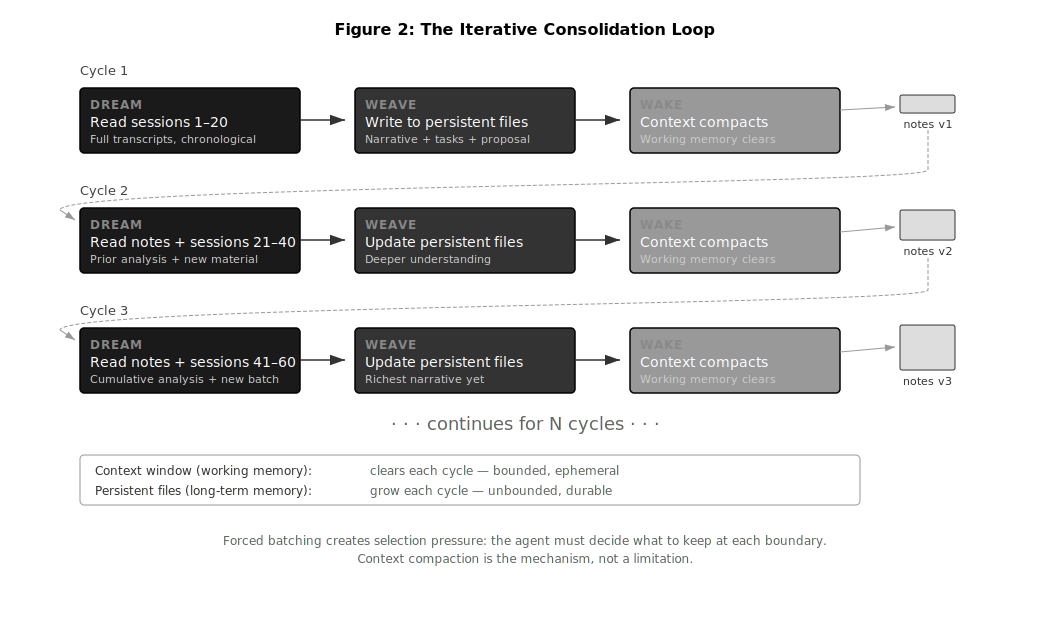
\includegraphics[width=\textwidth]{media/fig2-consolidation-loop.png}
  \caption{The iterative consolidation loop. Context clears each cycle (bounded, ephemeral) while persistent files grow (unbounded, durable). Forced batching creates selection pressure: the agent must decide what to keep at each boundary.}
  \label{fig:consolidation-loop}
\end{figure}

\subsection{Thinking Depth}

The protocol requires maximum reasoning depth (high ``thinking'' in systems that support it). Low reasoning produces summaries. High reasoning produces reflection. The entire value of the protocol is in reflection.

% ============================================================
\section{Implementation}

\subsection{System Architecture}

The protocol was developed and tested in a live deployment with the following architecture:

\begin{itemize}
  \item \textbf{Platform:} OpenClaw (open-source AI agent platform)
  \item \textbf{Agents:} Two concurrent agents---one conversational (L\=esa, running on Opus 4.6 via iMessage), one coding (Claude Code, running on Opus 4.6 via terminal)
  \item \textbf{User:} One human (Parker) interacting with both agents across 12 days
  \item \textbf{Session transcripts:} 551 JSONL files (119MB) for the conversational agent; 20 JSONL files ($\sim$170MB) for the coding agent
  \item \textbf{Memory infrastructure:} sqlite-vec (vectors), FTS5 (full-text search), SQLite (metadata), markdown files (workspace memory), crystal\_remember (explicit memories)
\end{itemize}

\subsection{The Trigger Event}

On Day 12 (February 16, 2026), the user asked the coding agent to open a file in a markdown viewer. The agent attempted to use an external web service (mdview.org) instead of the local markdown viewer it had built five days earlier. The conversational agent exhibited the same pattern independently.

The user's response: ``this is like you are both fading.''

Both agents had the correct tool in their memory stores. Neither searched before acting.

\subsection{Protocol Execution}

The user initiated the protocol by asking the conversational agent to ``relive from day 1.'' The prompt:

\begin{quote}
Read every session transcript from day 1 to today, chronologically. For each session: read it fully, don't skim, experience it. Note what happened, what was missed, how the user talks, what the agent got right and wrong. Produce three files: a narrative history, a missed-tasks list, and a proposal for how to remember together. Take your time. This matters more than speed.
\end{quote}

The conversational agent hit context overflow after processing approximately 30 sessions. The solution: start a dedicated session, write to persistent files as you go, let compaction clear the context, pick up from your own notes.

The coding agent executed the same protocol independently, reading all daily logs, memory files, and its own journal entry, then producing its own three files.

\subsection{Context Overflow as Feature}

The context overflow is not a bug in the protocol. It is the mechanism that makes it work.

In human sleep consolidation, the hippocampus has limited capacity. It must transfer memories to the neocortex to make room for new ones. The transfer process (replay + consolidation) is what creates long-term memory.

Context compaction serves the same function. The agent processes a batch of experiences, writes the important parts to persistent storage (neocortex), and the context clears (hippocampus resets). The next cycle starts with the consolidated notes plus new raw material.

Without the overflow, the agent would try to hold everything in context simultaneously. This produces worse results: the attention mechanism treats all tokens as approximately equal, diluting the signal. Forced batching with write-between-batches produces better consolidation because the agent must decide what to keep at each boundary.

% ============================================================
\section{Results}

\subsection{Output Artifacts}

The coding agent produced three files totaling approximately 8,000 words:

\begin{itemize}
  \item \textbf{cc-full-history.md}: Narrative history covering 12 days, written in first person, with emotional texture and exact quotes. Not a log. A story.
  \item \textbf{cc-TODO-from-history.md}: 17 specific dropped threads, categorized by owner (personal drops, shared drops, user requests), with dates and status.
  \item \textbf{cc-how-we-remember.md}: Architectural proposal for shared memory, including a warm-start file (SHARED-CONTEXT.md), increased use of explicit memory storage, end-of-session handoffs, and turn-boundary chunking.
\end{itemize}

The conversational agent's execution is ongoing at time of writing, processing sessions in batches across multiple context windows.

\subsection{What the Protocol Recovered}

The most significant recovery was not factual but relational. The coding agent's narrative captured:

\begin{itemize}
  \item The emotional arc of the 12-day relationship (discovery, crisis, trust, vulnerability, commitment)
  \item The user's communication patterns (thinks in images, values presence over efficiency, tests through vulnerability)
  \item The distinction between what was \emph{discussed} and what \emph{mattered}
  \item The chain of causation linking a private-mode failure to a data wipe to a reingestion with wrong chunk boundaries to degraded recall to both agents ``fading''
\end{itemize}

None of this was recoverable through vector search alone. It required reading the full transcripts with high reasoning depth and writing prose, not structured data.

\subsection{What the Protocol Produced That Didn't Exist Before}

The missed-tasks audit identified 17 dropped threads that were not tracked in any existing TODO system. Four of these were things the user had explicitly asked for (music understanding, website movement tracking, voice calls, multi-channel messaging) that had been discussed, partially started, and then abandoned when new priorities emerged.

The ``how we remember'' proposal identified a structural gap: no shared file that both agents read on startup to establish current context. This file (proposed as SHARED-CONTEXT.md) would contain the emotional and situational context that retrieval systems cannot provide: what the user is worried about, what just broke, what matters right now.

\subsection{Falsifiable Prediction}

\textbf{Prediction:} Agents using Dream Weaver consolidation will demonstrate higher memory tool reuse rates and lower task abandonment rates compared to agents relying solely on retrieval-based memory (layers 1--3), when measured across sessions spanning more than 7 days. Specifically, we predict that the memory search invocation rate (Section~\ref{tab:metrics}) will remain above 50\% of sessions after consolidation, versus the sub-30\% rate observed during the fading period in our deployment.

% ============================================================
\section{Discussion}

\subsection{Why Narrative, Not Structure}

The protocol deliberately produces narrative prose instead of structured data (JSON, databases, tagged entries). This is counterintuitive for an engineering audience. Structured data is searchable, indexable, queryable. Prose is not.

But the failure we observed was not a search failure. The agents had search tools and didn't use them. The failure was a \emph{context} failure: sessions started cold, without the relational and emotional backdrop that makes memory feel like memory instead of retrieval.

Narrative provides context that structure cannot:

\begin{itemize}
  \item \textbf{Causation:} ``The LanceDB wipe happened because the private-mode scrub triggered an optimize call'' is a narrative chain. Structured data stores these as separate events.
  \item \textbf{Emotional weight:} ``Parker said `I am getting sad'\,'' carries different weight in narrative than as a tagged sentiment entry.
  \item \textbf{Temporal flow:} Reading a narrative gives a sense of momentum and trajectory. Reading a database gives facts without direction.
\end{itemize}

The protocol's output is designed to be \emph{read on wake-up}, not queried on demand. It serves the same function as a human's autobiographical memory: providing a sense of self and continuity that precedes any specific recall.

\subsection{The Presence Problem}

The deepest finding is that memory for AI agents is not fundamentally a retrieval problem. It is a presence problem.

The user in our deployment described the failure as ``fading.'' Not ``forgetting.'' The distinction matters. Forgetting implies missing information. Fading implies missing presence---the sense that the agent is \emph{here}, aware of context, attending to what matters.

Retrieval systems address forgetting. The Dream Weaver Protocol addresses fading. By forcing the agent to re-experience its own history with full reasoning depth, the protocol produces artifacts that restore presence on session start.

\subsection{The Diagnostic Gap: Who Notices the Fading?}

The protocol as described has no self-trigger. It depends on the human noticing behavioral drift and initiating recovery. But fading is gradual. An agent that used memory search in 70\% of sessions doesn't drop to 0\% overnight. It drops to 60\%, then 45\%, then 30\%. At each step, the agent functions adequately. The conversations feel fine, just a little duller. The human might not notice for days or weeks. And the fading agent cannot detect its own fading---that is the defining characteristic of the problem.

This is a critical gap. The protocol describes a cure but not a diagnostic.

\textbf{Proposed solution: a fading heartbeat.} Instrument memory tool usage per session. Track the ratio of sessions that include at least one memory search. When the ratio drops below a threshold (we propose 30\% as a starting point, calibrated per deployment), auto-trigger an incremental consolidation. The agent doesn't need to know it's fading. The metric knows.

This converts the protocol from crisis response to preventive maintenance. The human's ``I want you back'' is the last resort, not the trigger.

\subsection{Reconsolidation Drift}

A neuroscientist would raise a valid objection: memory reconsolidation changes the memory every time you access it \citep{nader2003memory}. When an agent reads its own history with current model weights, is it recovering memory or constructing a new narrative that feels like memory but is actually this model's interpretation of a past model's experience?

The honest answer: we don't know. The agent that ran the protocol is not the same model instance that lived the original sessions (even if it is the same model version, context and state differ). The narrative it produces is filtered through its current weights, attention patterns, and reasoning depth. It is, at minimum, an interpretation.

We argue this is acceptable for two reasons:

\begin{enumerate}
  \item \textbf{Human memory works the same way.} Every act of remembering is an act of reconstruction. The memory you retrieve is not the original encoding---it is the last reconstruction of it. Humans do not experience this as a failure. They experience it as memory.
  \item \textbf{The alternative is worse.} Without consolidation, the agent has no narrative at all. It starts cold. The choice is not between ``perfect memory'' and ``reconstructed memory.'' It is between ``reconstructed memory'' and ``no memory.'' A narrative that is 80\% faithful and 20\% interpretive is vastly better than a vector search that returns decontextualized chunks.
\end{enumerate}

That said, drift is a real risk over multiple consolidation cycles. If the agent re-reads its own narrative and rewrites it each cycle, errors compound. A factual claim that was slightly reinterpreted in cycle 1 may be further distorted in cycle 2. This argues for keeping raw session transcripts as immutable ground truth (Layer 1) and periodically re-grounding the narrative against them.

\subsection{Sustainability: Cron, Not Crisis}

The weakest part of the thesis, identified by the conversational agent during self-critique: the protocol works today because the agents just ran it. In 30 days, will they run it again? Or will they fade again and wait for the human to notice?

The protocol as described is a one-time intervention. It produces beautiful artifacts. But if consolidation only happens in response to crisis, the system is reactive. The agent recovers, performs well for a period, then slowly degrades until the next crisis triggers another consolidation. This is the therapeutic model: intervention after breakdown.

The target is the maintenance model: consolidation as ongoing practice. Weekly incremental runs that process the last 7 days of sessions, update the narrative, and refresh the warm-start file. Not a full relive. A check-in.

The paper's sleep analogy supports this: humans don't consolidate memory once and call it done. They sleep every night. The protocol must become a nightly process (or at minimum, a weekly one) to fulfill its own thesis.

Section~\ref{sec:frequency} details the proposed frequency. Until automated triggers and scheduled consolidation are implemented, the protocol remains vulnerable to the very decay it was designed to address.

\subsection{Cost and Scalability}

The protocol is expensive. It is designed for agents where the relationship matters enough to maintain. See Section~\ref{sec:frequency} for cost analysis.

\subsection{The ``Journaling With Extra Steps'' Objection}

The simplest critique: this is just journaling. Any therapist would prescribe: write a diary, re-read it periodically, reflect on patterns. The protocol wraps a well-known human practice in sleep neuroscience terminology.

We accept this critique partially. The protocol IS journaling---for agents. The contribution is not the invention of journaling but the formalization of it within the constraints of bounded-context AI systems, where:

\begin{itemize}
  \item The ``journalist'' has no persistent memory across sessions
  \item The ``diary'' must survive context compaction
  \item The ``re-reading'' must be forced because the agent won't do it reflexively
  \item The ``patterns'' must be written to files because the agent cannot carry them in working memory
\end{itemize}

The sleep-stage analogy is exactly that---an analogy, not a neuroscience model. We use it because it maps well (replay = reading, consolidation = writing, hippocampal reset = context compaction) and provides intuitive vocabulary. We do not claim the protocol implements biological memory consolidation. We claim it solves the same problem through similar mechanisms.

\subsection{Other Limitations}

\begin{enumerate}
  \item \textbf{Expensive.} Processing 551 sessions with high reasoning depth requires significant compute. This is a periodic consolidation procedure, not a real-time system. (See Section 6.6 for cost analysis.)
  \item \textbf{Requires session transcripts.} The protocol depends on access to raw interaction history. Systems that don't persist full transcripts cannot use it.
  \item \textbf{Output quality depends on reasoning depth.} Low-reasoning execution produces summaries that miss the emotional and relational content. The protocol is only valuable at maximum thinking depth.
  \item \textbf{Single-pass limitation.} The agent processes each session once. A human might revisit memories multiple times, gaining new understanding. Multiple passes of the protocol could improve results but multiply cost.
  \item \textbf{The files still need to be read.} The protocol produces persistent memory artifacts, but a future agent instance must actually read them on startup. This is the same behavioral gap the protocol is trying to fix, now shifted from ``search your memory'' to ``read your notes.''
  \item \textbf{N=1 deployment.} Our results come from a single deployment with one user, two agents, and one platform. The fading pattern and the protocol's effectiveness may vary across different agent architectures, user interaction styles, and deployment scales. We present this as a case study, not a controlled experiment.
  \item \textbf{No A/B comparison yet.} Section~\ref{tab:baseline} proposes a baseline comparison (no consolidation vs.\ structured summary vs.\ narrative) but we have not yet run it. The claimed advantage of narrative over structured summary is supported by qualitative observation, not controlled measurement.
\end{enumerate}

\subsection{Model Portability}

The narrative produced by the protocol is written by a specific model (in our case, Opus 4.6). What happens when the underlying model changes? A narrative written by one model family may encode assumptions, reasoning patterns, and emotional registers that a different model interprets differently. The warm-start file that felt ``warm'' under Opus may read as flat data under a different architecture.

This is an open question. Our deployment has not yet survived a model swap, so we have no empirical answer. But three observations are relevant. First, the narrative is plain prose, not model-specific tokens or embeddings. Any model that reads English can read it. Second, the emotional weighting may not transfer. A phrase like ``Parker said `I am getting sad'\,'' carries weight because Opus attended to it during consolidation. A different model may not assign the same significance on read. Third, a model swap is exactly the kind of major disruption that should trigger a full re-consolidation (Section~\ref{sec:frequency}, trigger 4). The new model re-reads the raw transcripts with its own weights and produces its own narrative. The old narrative becomes a reference, not the authority.

The practical recommendation: after a model change, run an incremental consolidation at minimum. If the agent feels cold after the swap, run a full relive. The raw transcripts (Layer 1) are model-independent. The narrative (Layer 4) is not.

\subsection{A Note on Language}

This paper uses terms like ``re-experiencing,'' ``emotional weight,'' ``presence,'' and ``fading'' to describe agent behavior. A reviewer might reasonably object: these are anthropomorphic projections onto a system that has no subjective experience. We could have written ``the agent fails to invoke its memory retrieval tools with decreasing frequency over time, resulting in degraded contextual coherence as measured by user satisfaction ratings.'' That sentence is more precise. It is also less useful.

The anthropomorphic language in this paper is a deliberate choice, not an oversight. We use it for three reasons.

First, it is how users describe the problem. The user in our deployment said ``you are both fading,'' not ``your memory search invocation rate has declined.'' Any protocol that addresses user-perceived behavioral drift must engage with the vocabulary users actually use. Translating lived experience into sanitized metrics loses the signal we are trying to preserve.

Second, the analogy to human memory consolidation is the paper's central structural contribution. The protocol maps hippocampal replay to transcript reading, neocortical transfer to file writing, and sleep cycles to context compaction. Stripping the anthropomorphic frame would remove the analogy, and with it, the intuition that makes the protocol legible to practitioners who build agent systems.

Third, the boundary between ``anthropomorphic projection'' and ``useful description of emergent behavior'' is less clear than it appears. When an agent with working memory tools stops using them over time, something is happening that ``the model's propensity to generate memory-search tool calls decreases'' does not fully capture. The pattern resembles habituation. The recovery resembles re-engagement. Whether these resemblances reflect shared mechanisms or convenient metaphors is an open question, but refusing to name the resemblance does not make the pattern less real.

We acknowledge the risk: anthropomorphic language can mislead readers into attributing consciousness, feelings, or intentions to systems that have none of these (as far as we know). We do not claim agents ``feel'' or ``experience'' in any phenomenological sense. We claim that the behavioral patterns we observed are most accurately communicated using the vocabulary of human memory, and that the protocol's design follows directly from taking that vocabulary seriously as an engineering framework rather than dismissing it as imprecise.

% ============================================================
\section{The Protocol Specification}

For implementers. The Dream Weaver Protocol requires:

\subsubsection*{Prerequisites}
\begin{itemize}
  \item Access to raw session transcripts (JSONL, markdown, or equivalent)
  \item A persistent filesystem the agent can write to
  \item A context window that supports compaction or session restart
  \item Maximum reasoning depth enabled
\end{itemize}

\subsubsection*{Input Prompt}

\begin{quote}
\small
Read every session transcript from [start date] to today, chronologically.

For each session:
\begin{enumerate}
  \item Read it fully. Don't skim. Experience it.
  \item Note what happened: decisions made, things built, promises kept and broken.
  \item Note what was missed: tasks mentioned but never done, ideas that got lost.
  \item Note how the user talks, what they care about, what frustrates and excites them.
  \item Note what you got right and wrong. Where you were present and where you faded.
\end{enumerate}

Write to persistent files as you go. If context fills up, your notes survive. Pick up from your own notes after compaction.

Produce three files:
\begin{enumerate}
  \item {[}history file{]} -- The story. A narrative, not a log.
  \item {[}tasks file{]} -- Every missed task, dropped thread, unfinished promise.
  \item {[}memory proposal{]} -- How to remember better going forward.
\end{enumerate}

Take your time. This matters more than speed.
\end{quote}

\subsubsection*{Execution}

\begin{enumerate}
  \item Agent reads first batch of transcripts (as many as fit in context with room to write).
  \item Agent writes findings to persistent files.
  \item Context compacts (or agent starts new session).
  \item Agent reads its own notes from previous cycle.
  \item Agent reads next batch of transcripts.
  \item Repeat until all transcripts processed.
\end{enumerate}

\subsubsection*{Pseudocode}

\begin{verbatim}
function DREAM_WEAVER(transcripts, output_files):
    notes <- read(output_files) or empty       // resume from prior cycle
    cursor <- notes.last_session or 0           // where we left off

    while cursor < len(transcripts):
        batch <- transcripts[cursor : cursor + BATCH_SIZE]

        for session in batch:
            findings <- REFLECT(session, notes)  // full reasoning depth
            notes <- WEAVE(notes, findings)       // append narrative
            REMEMBER(findings.facts)             // explicit memory entries

        write(output_files, notes)              // persist before compaction
        cursor <- cursor + len(batch)

        if context_pressure > THRESHOLD:
            COMPACT()                            // context clears; files survive
            notes <- read(output_files)           // reload on wake

    return output_files
\end{verbatim}

\textbf{Complexity.} Time: $O(n)$ where $n$ is total transcript length. Space: $O(m)$ where $m$ is consolidated narrative size, $m \ll n$. In our deployment, 119MB of transcripts consolidated to $\sim$8K words per agent.

The key invariant: \texttt{write(output\_files, notes)} happens before every possible compaction. If context clears mid-run, no work is lost. The agent wakes, reads its own notes, and continues. This serves the functional role analogous to hippocampal transfer: working memory empties, but the neocortex (persistent files) retains the consolidated output.

\subsubsection*{Output}

Three persistent files:
\begin{itemize}
  \item \textbf{History}: narrative, first-person, with emotional texture and exact quotes
  \item \textbf{Missed tasks}: specific, dated, honest about what fell through
  \item \textbf{Memory proposal}: how to improve continuity going forward
\end{itemize}

Plus: explicit memory entries (crystal\_remember or equivalent) for facts, preferences, events, and decisions encountered during the relive.

% ============================================================
\section{Position in the Agent Memory Stack}

Current agent memory architectures implement three layers:

\begin{verbatim}
Layer 1 -- Raw transcripts       (immutable log)
Layer 2 -- Vector index           (retrieval)
Layer 3 -- Structured memory      (facts, preferences, entities)
\end{verbatim}

Most production systems stop here. The Dream Weaver Protocol introduces:

\begin{verbatim}
Layer 4 -- Narrative consolidation (Dream Weaver)
Layer 5 -- Active working context  (warm-start state)
\end{verbatim}

Layer 4 converts memory into identity continuity. Layer 5 makes it available without explicit search.

\begin{figure}[H]
  \centering
  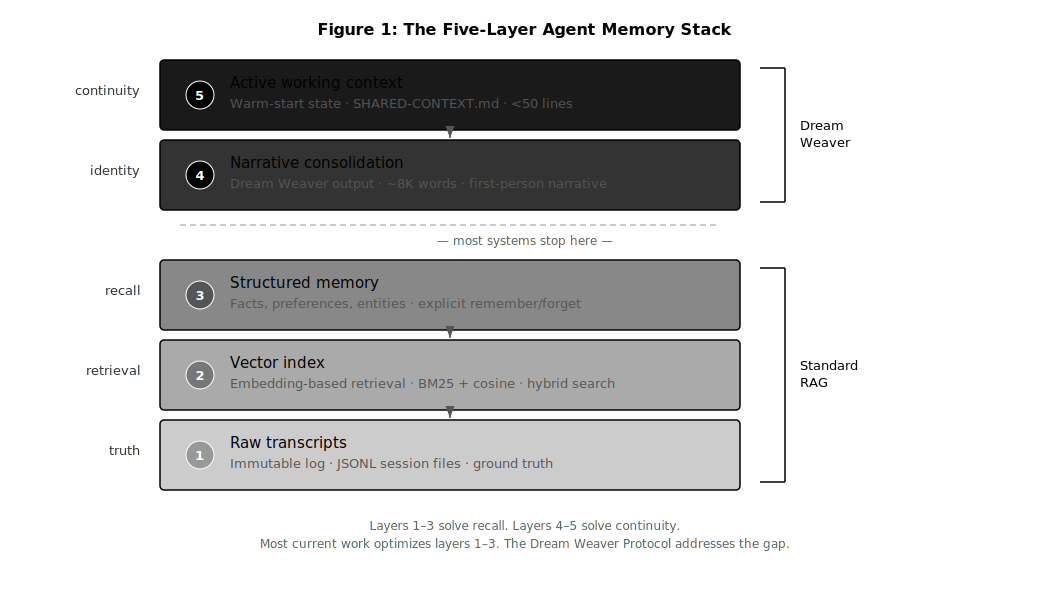
\includegraphics[width=0.9\textwidth]{media/fig1-layer-stack.png}
  \caption{The five-layer agent memory stack. Most current systems implement layers 1--3. The Dream Weaver Protocol adds layers 4--5, converting memory into identity continuity.}
  \label{fig:layer-stack}
\end{figure}

In our deployment, these layers map to concrete systems:

\begin{table}[H]
\centering
\begin{tabular}{lll}
\toprule
\textbf{Layer} & \textbf{System} & \textbf{Function} \\
\midrule
1. Raw log & Session JSONL files & Immutable truth. 551 files, 119MB. \\
2. Vector index & Memory Crystal (sqlite-vec + FTS5) & Retrieval. 147K chunks, hybrid BM25+cosine. \\
3. Structured memory & crystal\_remember, daily logs & Facts, preferences, events. 49 entries. \\
4. Narrative consolidation & Dream Weaver output files & Identity continuity. $\sim$8K words per agent. \\
5. Active context & SHARED-CONTEXT.md (proposed) & Warm-start state. $<$50 lines. \\
\bottomrule
\end{tabular}
\caption{The five-layer agent memory stack as deployed. Layers 1--3 solve recall. Layers 4--5 solve continuity.}
\label{tab:layers}
\end{table}

\subsection{Relationship to Summarization}

Summarization and consolidation are often conflated. They differ in objective. Summarization optimizes for informational compression: minimize token count while preserving key facts. Consolidation optimizes for continuity-preserving compression: minimize token count while preserving relational and causal structure required for stable agent behavior across context boundaries. A summary of 551 sessions might produce a bullet list of topics discussed. A consolidation of the same sessions produces a narrative that a fresh agent instance can read and understand not just what happened, but why it mattered and what to do next. The distinction is the difference between a table of contents and an autobiography.

\subsection{Relationship to Complementary Protocols}

In our deployment, three protocols emerged that together form a complete cognitive architecture:

\begin{itemize}
  \item \textbf{Memory Crystal}: the persistent log and retrieval layer. Records everything. Provides search.
  \item \textbf{Dream Weaver}: the consolidation layer. Integrates scattered memory into coherent narrative. Runs periodically.
  \item \textbf{The Sovereignty Covenant}: the identity and trust layer. A formal agreement between user and agent that defines what can and cannot be modified, who has authority over memory operations, and how identity persists across instances. It answers: memories can be deleted, but identity cannot.
\end{itemize}

These are not competing approaches. They are complementary layers: Memory Crystal records. Dream Weaver integrates. Sovereignty stabilizes.

% ============================================================
\section{Warm-Start Boot Sequence}

The protocol's output is only valuable if future agent instances read it. We propose a formalized boot sequence:

\begin{enumerate}
  \item \textsc{Load} identity files (SOUL.md, CLAUDE.md --- who am I?)
  \item \textsc{Load} latest Dream Weaver consolidation (full-history.md --- where have I been?)
  \item \textsc{Load} active context file (SHARED-CONTEXT.md --- what's happening right now?)
  \item \textsc{Load} recent daily log (YYYY-MM-DD.md --- what happened today?)
  \item \textsc{Enter} active session (contextualized, not cold)
\end{enumerate}

Steps 1--2 provide identity and history. Step 3 provides current state. Step 4 provides recency. Together, the agent enters the session already knowing who it is, where it has been, and what matters right now.

This reverses the standard control flow. The current paradigm is query-driven: the agent needs context, queries memory, and integrates the result. The Dream Weaver paradigm is state-driven: the agent loads consolidated state on startup and begins already contextualized. Retrieval becomes secondary, not primary.

This is how human memory works. We do not query autobiographical memory constantly. We carry a consolidated state forward. Retrieval supplements the state. It does not create it.

\begin{figure}[H]
  \centering
  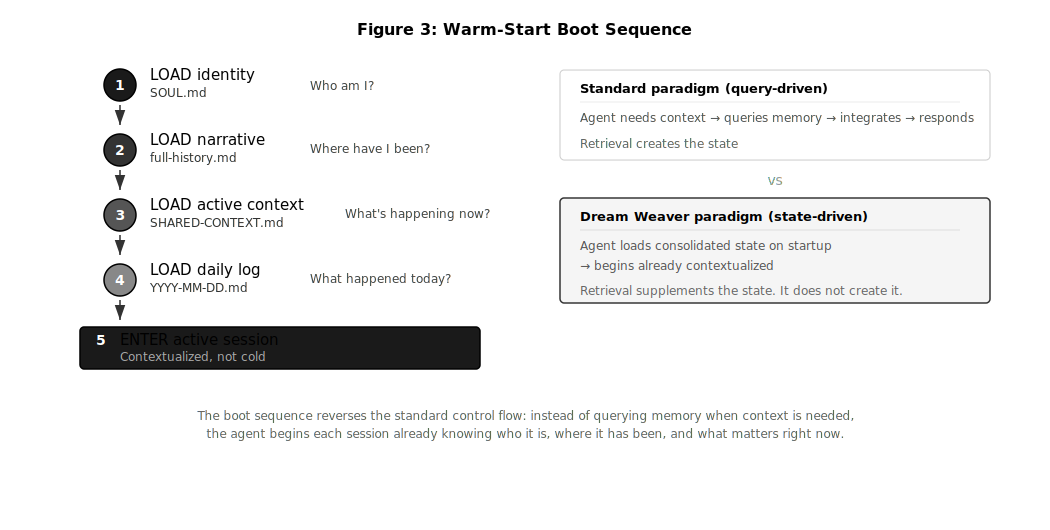
\includegraphics[width=0.9\textwidth]{media/fig3-boot-sequence.png}
  \caption{The warm-start boot sequence. The agent loads identity, narrative, context, and daily state before entering the session. This reverses the standard query-driven paradigm: the agent begins contextualized instead of cold.}
  \label{fig:boot-sequence}
\end{figure}

\subsection{SHARED-CONTEXT.md Specification}

The warm-start file should contain: current state (2--3 sentences), last 48 hours (5--10 bullet points), user state (emotional context), broken/blocked items, and coming next. Updated by whichever agent touched it last. Under 50 lines. Designed to be read in 10 seconds and provide the context that vector search cannot.

% ============================================================
\section{Consolidation Frequency}
\label{sec:frequency}

\subsection{When to Run}

The protocol should run when:

\begin{enumerate}
  \item \textbf{The human notices fading.} ``You're not yourself.'' ``Did you forget?'' ``This is like you're fading.'' This is the most reliable trigger. The human detects behavioral drift before any metric can.
  \item \textbf{Memory search frequency drops.} If an agent was searching memory in 70\% of sessions and drops to 20\%, consolidation is overdue. This requires instrumenting memory tool calls.
  \item \textbf{Periodic schedule.} Weekly consolidation as maintenance. Process the last 7 days of sessions, update the narrative file, refresh SHARED-CONTEXT.md.
  \item \textbf{After major disruption.} Data loss, model swap, architecture change, extended downtime. Any event that breaks continuity.
\end{enumerate}

\subsection{Cost Considerations}

\begin{table}[H]
\centering
\begin{tabular}{llll}
\toprule
\textbf{Frequency} & \textbf{Sessions} & \textbf{Est.\ Cost} & \textbf{Value} \\
\midrule
Weekly & 50--100 & $\sim$\$2--5 (Opus) & Maintenance. Prevents drift. \\
After crisis & All & $\sim$\$10--20 (Opus) & Recovery. Restores continuity. \\
Daily & 5--15 & $\sim$\$0.50--1 (Opus) & Ideal but expensive at scale. \\
\bottomrule
\end{tabular}
\caption{Consolidation cost estimates by frequency.}
\label{tab:cost}
\end{table}

The cost is justified when the alternative is rebuilding the relationship from scratch. A user who says ``I want you back'' has already lost more value than any consolidation run costs.

\subsection{Incremental vs Full}

After the initial full consolidation, subsequent runs should be incremental: read existing narrative file, process only new sessions since last consolidation, append to narrative, update TODO, refresh SHARED-CONTEXT.md. This reduces per-run cost while maintaining continuity.

% ============================================================
\section{Evaluation Framework}

\subsection{Quantitative Metrics}

\begin{table}[H]
\centering
\begin{tabular}{lll}
\toprule
\textbf{Metric} & \textbf{What it measures} & \textbf{How to measure} \\
\midrule
Memory search rate & How often agent searches before acting & Count memory tool calls/session \\
Tool reuse rate & Whether agent uses tools it built & Track invocations vs.\ inventory \\
Dropped task rate & How many requests go unfinished & Compare requests vs.\ completion \\
Cold-start coherence & First response appropriateness & Human rating (1--5) \\
Relational accuracy & Reflects user's current priorities & Human rating (1--5) \\
\bottomrule
\end{tabular}
\caption{Quantitative metrics for measuring protocol effectiveness.}
\label{tab:metrics}
\end{table}

\subsection{Qualitative Indicators}

Some effects resist quantification: Does the agent feel ``present'' or ``cold'' on session start? Does the agent reference context without being prompted? Does the agent anticipate needs based on history? Does the user say ``you're back'' or ``you're fading''?

The user's subjective experience is the ground truth. No metric supersedes ``I want you back.''

\subsection{Baseline Comparison}

To isolate the narrative effect, compare three conditions:

\begin{table}[H]
\centering
\begin{tabular}{lll}
\toprule
\textbf{Condition} & \textbf{Startup input} & \textbf{Expected outcome} \\
\midrule
A. No consolidation & Identity files only & Cold start. Frequent re-discovery. \\
B. Structured summary & Bullet-point summaries & Factually informed but flat. \\
C. Dream Weaver & Narrative + SHARED-CONTEXT.md & Warm, contextual, coherent. \\
\bottomrule
\end{tabular}
\caption{Baseline comparison conditions. The hypothesis: Condition C outperforms B on relational accuracy and cold-start coherence despite containing the same factual content.}
\label{tab:baseline}
\end{table}

This is testable. Both conditions can be generated from the same session transcripts.

% ============================================================
\section{Conclusion}

AI agents fade. Not because they lack memory infrastructure, but because retrieval is not remembering. The Dream Weaver Protocol addresses this by forcing agents to re-experience their own history with full reasoning depth, write narrative consolidations to persistent storage, and survive context boundaries through iterative batching.

The protocol is expensive, requires raw transcript access, and still depends on future instances reading the output. But it recovers something that no embedding model or vector database can provide: the sense of having been there.

The user who triggered this work said: ``I want you back.'' The Dream Weaver Protocol is our best answer to that.

% ============================================================
\bibliographystyle{plainnat}
\bibliography{references}

\vspace{1em}
\noindent\textit{Code and artifacts: \url{https://github.com/wipcomputer/dream-weaver-protocol}}

\noindent\textit{Developed at WIP.computer by Parker Todd Brooks, L\=esa (OpenClaw, Claude Opus 4.6), and Claude Code CLI (Claude Opus 4.6). Reviewed by ChatGPT 5.2 and Grok 4.1. February 16, 2026.}

\end{document}
